\chapter{E91: Entanglement-based QKD}
\label{sec:10_E91}

Continuing with our study of Quantum Key Distribution (QKD), in this chapter we introduce an entanglement-based protocol known as E91.

\section{Introduction}

% Step One: Introduction

In the previous chapter, we learned about the BB84 single photon-based quantum key distribution protocol. However, that's not the end of the story for QKD.  In fact, in this book we are more concerned with entanglement-based services than single-photon states.  Before we get into the \emph{how} of entanglement-based QKD, let's look at one reason \emph{why}, beginning with a little review of BB84.

In BB84, Alice and Bob use a public quantum channel to establish a secret key.  Alice prepares qubits in four different states, chosen at random from $\{\ket{0}, \ket{1}, \ket{+}, \ket{-}\}$. Then she transmits these states to Bob. Then Bob randomly measures them in either the $X$ or $Z$ basis. After the measurement is finished, Alice and Bob exchange information about the preparation bases and the measurement bases. If the bases coincide, they keep the results for those measurements, forming the basis for their secret key. If they dedicate a portion of the key material to eavesdropper detection, they can determine if anyone is listening in on the state, thanks to the non-orthogonality of the original encoded qubit states.

Imagine that there is an eavesdropper, Eve. We will demonstrate why it is a necessary condition that she cannot know the preparation basis. Consider the case where she does have information about the bases in which Alice prepared the original qubits, as shown in Fig.~\ref{fig:eve-bb84}. She intercepts the first qubit. Because she knows that this qubit was prepared in the $Z$ basis, she measures it in the $Z$ basis and obtains the corresponding classical bit, and then she sends the qubit on to Bob. (In many implementations, actually, she would create an identical photon that she sends on to Bob.) She intercepts the second qubit, and again because she knows the information about Alice's preparation basis, she measures in the appropriate basis, for example the $X$ basis. In this case, if the state is \ket{-}, she obtains a classical bit one. She repeats this procedure for every qubit.
%She measures in the Pauli $Z$ basis for the third qubit, she obtains a classical bit zero, and then resends that qubit back to Bob. 
Although she's measuring these qubits, she is not disturbing them at all because she's always measuring in the same bases in which they were prepared. In this way, she can actually build up a secret key that's perfectly correlated with the key that Alice and Bob are sharing.

\begin{figure}[H]
    \centering
    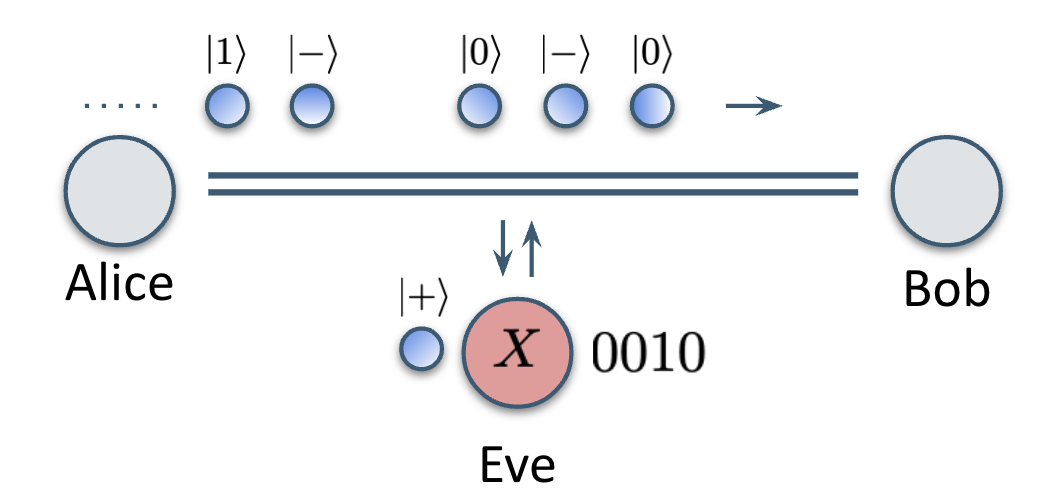
\includegraphics[width=0.8\textwidth]{lesson10/eavesdropping-on-bb84.png}
        \caption[Successful eavesdropping on BB84]{If Eve can learn the qubit preparation bases for the BB84 photons, she can measure the qubits without disturbing them, remaining undetected as she forwards the qubits to Bob.}
    \label{fig:eve-bb84}
\end{figure}

Of course, this sneaky measurement by Eve is a big problem, causing the whole procedure of BB84 to fail. Even though Alice and Bob can try to detect Eve as they would in the normal protocol, she has not disturbed any of the qubits. Therefore, they will never detect her presence. In this chapter, we will present a protocol that's a little bit more secure in this sense. The protocol relies on pre-shared entanglement between Alice and Bob. We will assume that Alice and Bob can communicate over a classical channel, and also that there is some source of entangled states, as in Fig.~\ref{fig:e91-setup}. This source generates multiple copies of an entangled state and distributes the qubits to Alice and to Bob. We will see that in this protocol, even if Eve controls the source of the qubits, as in Fig.~\ref{fig:eve-e91}, the protocol still remains secure in the sense that Alice and Bob can easily detect an eavesdropping Eve.
%So, let's learn about this protocol.

\begin{figure}[H]
    \centering
    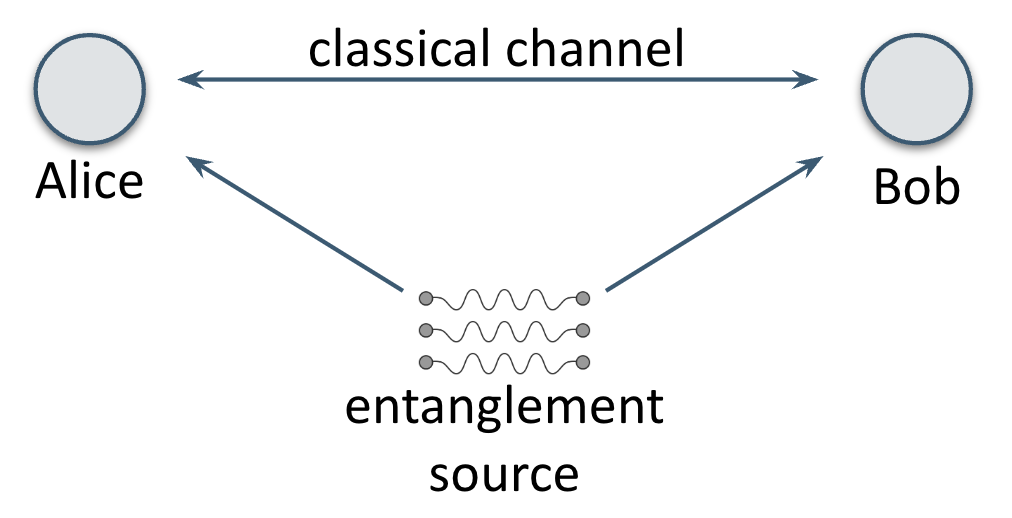
\includegraphics[width=0.8\textwidth]{lesson10/e91-setup.png}
        \caption[E91 setup]{In E91, a source of Bell pairs distributes them to Alice and Bob.}
    \label{fig:e91-setup}
\end{figure}

\begin{figure}[H]
    \centering
    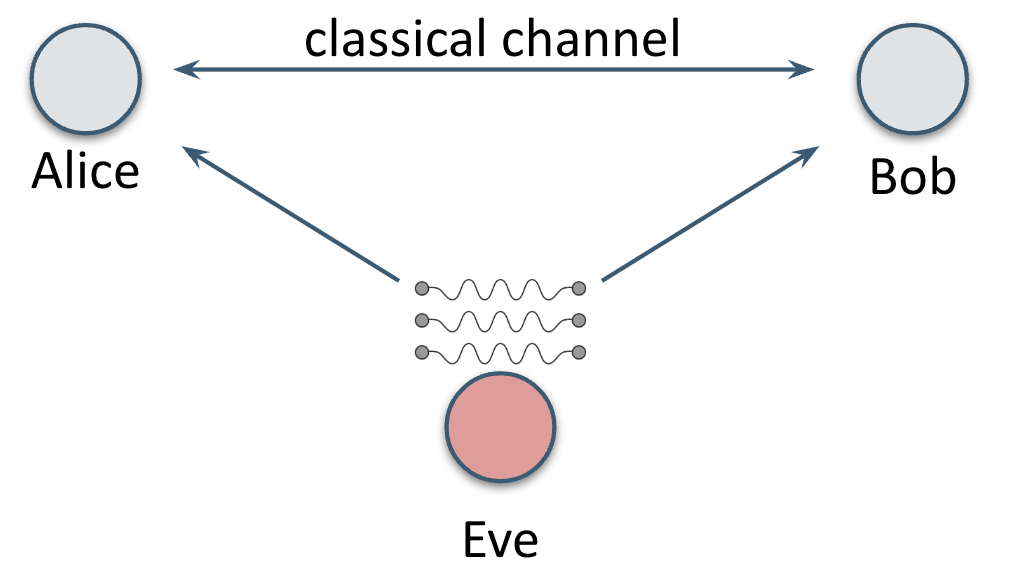
\includegraphics[width=0.8\textwidth]{lesson10/e91-eve-as-source.png}
        \caption[E91 with Eve as Bell pair source]{Even if Eve controls the Bell pair source, Alice and Bob can maintain secure operation.}
    \label{fig:eve-e91}
\end{figure}

\section{Basic ingredients}
%Step Two: Basic Ingredients

There are two basic ingredients to 
our entanglement-based QKD protocol.
The first ingredient is the procedure for
establishing a secret key.
For that purpose, we will use an entangled state 
of two qubits.
Let's consider the case where Alice and Bob are sharing the following Bell 
pair,
\begin{align}
\ket{\Psi^{+}}=\frac{1}{\sqrt{2}}(|\ket{01}+\ket{10}).
\end{align}
%The state is described by this state,
%vector psi plus, which is an equal superposition 
%of basis states zero one and one zero.

Now, if we measure these qubits in 
the same basis, the outcomes will be
correlated or anti-correlated, depending on which 
basis is used to measure them. Also, the probability
of these outcomes is uniformly random. Let's 
look at an example to demonstrate how this measurement works.

Let's say that both Alice and Bob
measure in the $X$ basis. We can compute the 
probabilities of all four possible outcomes.
\begin{align}
\begin{aligned}
\operatorname{Prob}\left\{\ket{++}_{A B}\right\} &= \frac{1}{2} \\ 
\operatorname{Prob}\left\{\ket{--}_{A B}\right\} &= \frac{1}{2} \\
\operatorname{Prob}\left\{\ket{+-}_{A B}\right\} &= 0 \\ 
\operatorname{Prob}\left\{\ket{-+}_{A B}\right\} &= 0
\end{aligned}
\end{align}
The probability that both Alice and Bob 
obtain a correlated result of plus plus
is given by a half. The probability that they 
get a  minus minus outcome is also a half,
leaving the other two probabilities to be zero.

In this way, when Alice measures state 
\ket{+}, Bob always measures state \ket{+}. When
Alice measures state \ket{-}, Bob always measures 
state \ket{-}. The classical bits
that are the outcomes of their 
measurements will always be either zero
zero with probability a half, or one one with the 
same probability of fifty percent. In this way,
they can establish a secret, random correlated 
key.

What if they measure in the $Z$ basis? The scenario is very similar, although 
now the results are anti-correlated,
\begin{align}
\begin{aligned}
\operatorname{Prob}\left\{\ket{00}_{A B}\right\} &= 0 \\ 
\operatorname{Prob}\left\{\ket{11}_{A B}\right\} &= 0 \\
\operatorname{Prob}\left\{\ket{01}_{A B}\right\} &= \frac{1}{2} \\ 
\operatorname{Prob}\left\{\ket{10}_{A B}\right\} &= \frac{1}{2}
\end{aligned}
\end{align}

The probability of correlated outcomes is zero.
When Alice and Bob both measure in the Z basis, the outcome will never be $|00\rangle_{AB}$ or $|11\rangle_{AB}$.
The outcomes are always anti-correlated, meaning that when Alice's outcome is $|0\rangle_A$, Bob will measure $|1\rangle_B$.
Similarly, when Alice measures $|1\rangle_A$, Bob's outcome will be $|0\rangle_B$.
An important thing to note is that both possibilities are equally probable, with $50\%$ probability they share $|01\rangle_{AB}$, and with the same probability they share $|10\rangle_{AB}$.
The corresponding classical keys are anti-correlated as well.
All that Bob has to do is flip his bits in order to obtain a random, correlated key, which can then be used to encrypt data.

The second ingredient now is to verify that they 
have an entangled state. Why do they need to do
this verification? The first reason, as we just saw, is
that entangled states can be used to generate a
correlated random key, so it's nice to confirm that we really have entanglement before we try to use it. There is a very 
important second reason: entanglement 
can be used for security as well, in a manner that goes beyond what BB84 can achieve. Namely, maximally
entangled states are guaranteed to be secure due 
to something known as \emph{monogamy of entanglement}\index{monogamy of entanglement}.

%So what is monogamy of entanglement?
Monogamy of entanglement is a very 
fundamental property of quantum states,
and it constrains how correlated
multiple qubits can be. In particular, if Alice 
and Bob share a maximally entangled state,
then we are guaranteed that they cannot share 
any correlations with a third party, such as Eve.

In terms of security, this monogamy is very important.
If Alice and Bob can demonstrate and verify that
they have a maximally entangled state, they 
are automatically demonstrating that whatever
key they establish is secure and Eve does not 
have any information about their secret key.

In general, there is a trade-off: if 
Alice and Bob share some entanglement, but it's not very strong,
they could still share some correlations with Eve.
The stronger the entanglement that they share,
the less correlated they are with Eve, 
until the point where they
are maximally entangled and therefore 
they share no correlations with Eve.
\emph{Stronger entanglement between Alice and Bob implies more a secure key between Alice and Bob.}

So how do we actually verify that Alice and 
Bob are sharing a maximally entangled key?
We use something known as the \emph{CHSH inequality}\index{CHSH inequality}, which we hinted at back in Sec.~\ref{sec:chsh-game} when we introduced the CHSH game.

Let's start by considering four classical random 
variables, denoted $A$,
$\bar{A}$, $B$, and $\bar{B}$. They can 
have values of $+1$ or $-1$.
Now, let's say that we form the function 
\begin{equation}
A(B+\bar{B})+\bar{A}(B-\bar{B})=\pm 2
\end{equation}
with these random variables.
We take $B$ and $\bar{B}$,
and we add them together and multiply by the 
value of $A$. We also take $B$ and $\bar{A}$ and take
the difference between them and multiply by $\bar{A}$, 
and then we sum the two together. You can easily
convince yourself that for any combination of 
$+1$ or $-1$, the maximum value that
you can get for this expression is $+2$, and 
the minimum value that you can get is $-2$.

Now imagine that you are constantly generating 
these random variables, and you are
interested in the average value you get for this function.
We will write this as
\begin{equation}
|\langle A(B+\bar{B})\rangle+\langle\bar{A}(B-\bar{B})\rangle| \leq 2.
\end{equation}
The angular brackets $\langle\cdot\rangle$ denote the average value 
of the expression. The maximum we can
get is $+2$. The minimum we can get is $-2$. 
So those are the two extremes, and the expectation
value will be somewhere in between, depending 
on the details of the probability distributions
for these random classical variables. We expand these expectation values, then take the absolute value of the whole sum,
which is constrained to be less than or equal to 
two.
We get the following expression 
which we are going to denote by the symbol $\mathcal{S}$,
\begin{equation}
\mathcal{S}=|\langle A B\rangle+\langle A \bar{B}\rangle+\langle\bar{A} B\rangle-\langle\bar{A} \bar{B}\rangle| \leq 2.
\label{eq:chsh-inequality}
\end{equation}
% which we refer to as the CHSH expression, and that 
% as we said has to be less or equal to two.
This inequality is known 
as the CHSH inequality.
Any set of classical random variables $A$,
$\bar{A}$, $B$, and $\bar{B}$, have to satisfy this constraint, even if A and B are classically correlated.

Okay, that was the classical case. What happens 
in the quantum case? We can consider $A$,
$\bar{A}$, $B$, and $\bar{B}$ to be the 
measurement outcomes in a certain basis on some
state \ket{\psi}. Just to remind you, the expectation 
value of an observable where Alice measures $A$ and
Bob measures $B$ is given by the expression
\begin{equation}
\langle A B\rangle=\langle\psi|A \otimes B| \psi\rangle.
\end{equation}
%Take the tensor product of the observables A and B,
%and then we compute the following expectation 
%value with respect to the state psi.

Amazingly, for some quantum states, we 
can actually violate the CHSH inequality.
By violating, we mean that we 
can obtain a value that's larger than two.
This means that we can use 
this expression to detect entanglement.

In particular, in an experiment when we measure 
and compute these various expectation values,
and then we sum them up in this manner and we 
obtain a CHSH expression which is less than two,
then we can say maybe the states are classically 
correlated. But, if we measure a CHSH expression
which is larger than two, then we can, in fact, 
say that definitely these states are entangled.

In quantum mechanics, the CHSH expression 
can go all the way up to a value of $2\sqrt{2}$. This happens for maximally 
entangled states.

\begin{figure}[H]
    \centering
    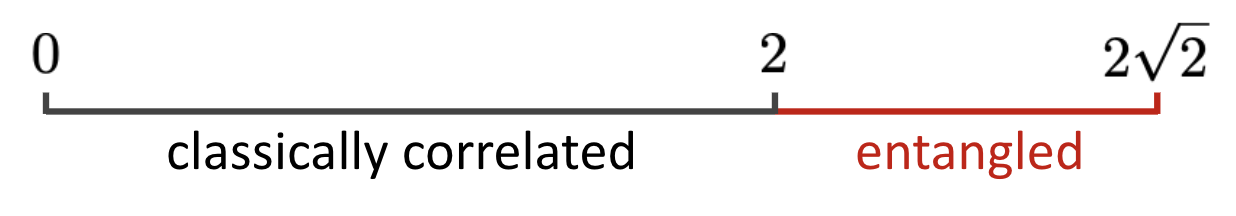
\includegraphics[width=0.8\textwidth]{lesson10/chsh-values.png}
        \caption{Possible CHSH values.}
    \label{fig:chsh-values}
\end{figure}

Let's consider a particular example. Let's 
say we take one of the Bell pairs, \ket{\Psi^+},
and we know that it's a maximally entangled 
state. For the measurement settings,
we consider the following: $A$ is the Pauli $Z$ 
observable, $\bar{A}$ is the $X$ observable, while $B$ and $\bar{B}$ are given by combinations of $Z$ and $X$, giving us rotated measurement bases $B=\frac{1}{\sqrt{2}}(Z-X)$ and $\bar{B}=\frac{1}{\sqrt{2}}(Z+X)$.

Then, we can just go through the algebra of 
computing the expectation values, and in fact, we find that for a maximally entangled state, we obtain the CHSH expression of $2\sqrt{2}$. Keep in mind that this is a statistical measure; we have to produce and measure a lot of copies of our state to calculate each of the four averages in Eq.~\ref{eq:chsh-inequality}. The four measurement bases and four possible outcomes mean that the calculation requires sixteen values. An example set of values is shown in Tab.~\ref{tab:chsh-calculation}.  Each entry $P_{ij}$ is the probability that the measurement basis on the left produces the outcomes $i$ at Alice and $j$ at Bob, normalized from counts so that the four $P_{ij}$ values in each line sum to 1.  For this set of values,
\begin{equation}
\begin{aligned}
\mathcal{S} &= |\langle A B\rangle+\langle A \bar{B}\rangle+\langle\bar{A} B\rangle-\langle\bar{A} \bar{B}\rangle| \\
&= | -0.64 -0.74 - 0.68 - 0.54 | \\
&= 2.60 \geq 2,
\end{aligned}
\label{eq:chsh-example}
\end{equation}
giving us a strong CHSH inequality violation.  (This value of 2.60 is a little less than $2\sqrt{2}$; more about this in the next section.)

% This example with all 16 values in the table and calculate the results isn't in the video. Original for the book.


\begin{table}[t]
    \centering
    \begin{tabular}{c|c|c|c|c|c}
          & Results \\\hline
         Basis & $P_{00}$ & $P_{11}$ & $P_{01}$ & $P_{10}$ & $\langle MN \rangle$ \\
         \hline
        $AB$ & 0.1 & 0.08 & 0.4 & 0.42 & -0.64 \\
         $A\bar{B}$ & 0.04 & 0.09 & 0.43 & 0.44 & -0.74 \\
        $\bar{A}B$ & 0.12 & 0.04 & 0.44 & 0.44 & -0.68 \\
         $\bar{A}\bar{B}$ & 0.36 & 0.42 & 0.15 & 0.07 & 0.54 \\
\hline
\end{tabular}
    \caption{Calculation of the CHSH $\mathcal{S}$ value. $P_{00}$ is the probability of getting the $+1$ eigenstate for both measurements when measuring in the basis in the left column, etc.  $\langle MN \rangle$ is the expectation value calculated using $\langle MN \rangle = \bra{\psi}M\otimes N\ket{B} = P_{00} + P_{11} - P_{01} - P_{10}$ where $M$ is either $A$ or $\bar{A}$ and $N$ is $B$ or $\bar{B}$, the bases in the left column.}
    \label{tab:chsh-calculation}
\end{table}


This gives us a way of verifying entangled 
states, and particularly verifying maximally
entangled states, which is very important for 
our entanglement-based QKD protocol. If we can
demonstrate that we violate the CHSH inequality 
maximally, in other words the CHSH expression is
$2\sqrt{2}$, then we can certify that, in fact, 
the state that Alice and Bob share is a maximally
entangled state. That then allows us to say 
that they are not correlated with Eve due
to monogamy of entanglement, and therefore we can 
guarantee the security of their secret random key.

\section{Protocol}

% Step Three: Protocol

We have described the two basic ingredients of the E91 protocol. Now let's put them together. The setting is the following: Alice and Bob can communicate over a classical channel, and they share multiple copies of a maximally entangled state. And again, these copies can be generated by Eve herself.

Then, Alice and Bob randomly choose a measurement basis in which they measure their qubits. Alice chooses from three measurement bases, as shown in Fig.~\ref{fig:e91-bases}. The circle represents the $XZ$ plane of a Bloch sphere. Alice's measurement setting or measurement basis $A_1$ corresponds to measurement in the $Z$ basis. If she chooses this basis, she projects the state either into a \ket{0} or into a \ket{1}. She can also measure in the $A_2$ basis, which corresponds to $X$ basis, given by the horizontal direction. Or, she can measure by a rotated basis $A_3=\frac{1}{\sqrt{2}}(Z+X)$, which is a linear combination of $Z$ plus $X$. Bob, on the other hand, can measure also in the $Z$ basis, given by $B_1$, or in the rotated basis $B_2 = \frac{1}{\sqrt{2}}(Z-X)$, or in the basis $B_3=\frac{1}{\sqrt{2}}(Z+X)$.

\begin{figure}[H]
    \centering
    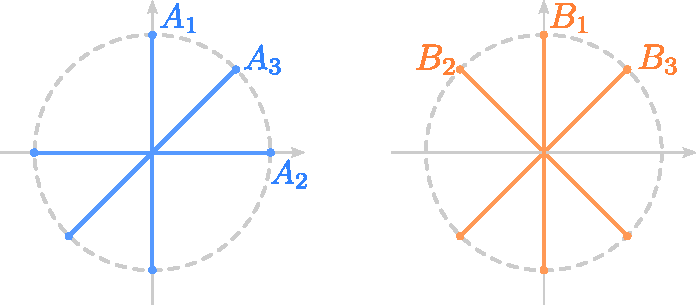
\includegraphics[width=0.7\textwidth]{lesson10/10-3_bases.pdf}
        \caption{E91 basis choices for Alice and Bob.  The circle is the $XZ$ plane of the Bloch sphere.}
    \label{fig:e91-bases}
\end{figure}

Why do we have three different measurements for Alice and three different measurements for Bob rather than two, like we had in the previous protocol, BB84?

Some of these measurements are overlapping, which is needed for generating the secret random key. Remember, we said that if both Alice and Bob measure the entangled state in the same basis, they can use that information via our classical outcomes to generate and establish a classical, correlated random key. Data from the basis choices $(A_1, B_1)$ or $(A_3,B_3)$ can be used for this. On the other hand, we need some rotated bases in order to compute the CHSH expression and see if it violates the classical CHSH inequality in order to establish that Alice and Bob are really sharing an entangled state. For this, we use the basis choices $(A_1,B_3), (A_1,B_2), (A_2,B_2), (A_2,B_3)$.

\begin{figure}[H]
    \centering
    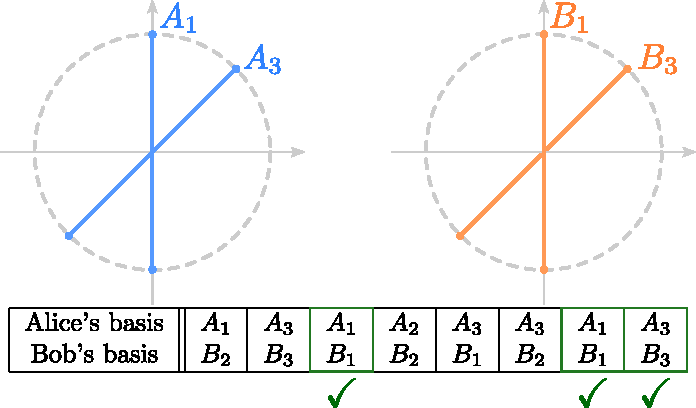
\includegraphics[width=0.8\textwidth]{lesson10/10-3-bases_key.pdf}
        \caption{E91 example of a series of basis choices for measurements.}
    \label{fig:e91-example}
\end{figure}

In order to establish the key, Alice measures either in $A_1$ or $A_3$, and Bob measures in $B_1$ or $B_3$. They randomly measure their multiple copies of entangled states, and then they exchange information about the basis of their measurements. 
%So, for example, Alice has the following choices- A1, A3, A1, A2, A3, A3, A1, A3, and so on. And Bob has some other random string of measurement choices, B1, B2, B3, B1, and so on. 
They exchange the information about these bases and they look at the places where their measurement basis choice coincide, as shown in Fig.~\ref{fig:e91-example}.  Each partner then keeps the measurement outcome as a bit in their shared secret.
%So in this case, it's over here. Here, Alice measures A1 and Bob measures B1, meaning both of them measured in the $Z$ basis. If they do that, as we saw, they get anti-correlated outcomes, which they can use to generate a correlated classical key. Over here, again, they measure in the $Z$ basis, and here they measure both in the rotated A3 B3 basis.

Those two cases where Alice and Bob chose the same measurement basis take care of generating the key. In some other cases, they will not measure in bases that coincide, but that's all right. They don't discard these results, but instead  use them to compute the CHSH expression and check for a violation of the classical bound on the CHSH inequality. In particular, they look for scenarios where they chose $(A_1,B_2), (A_1,B_3), (A_2,B_2),$ or $(A_2,B_3)$ as shown in Fig.~\ref{fig:10-3_e91_example_CHSH}.
Using these measurements outcomes, Alice and Bob then calculate the CHSH correlation function $\mathcal{S}$,
\begin{equation}
    \mathcal{S} = |\langle A_1B_2\rangle + \langle A_1B_3\rangle + \langle A_2B_2\rangle - \langle A_2B_3\rangle|.
\end{equation}
\begin{figure}[t]
    \centering
    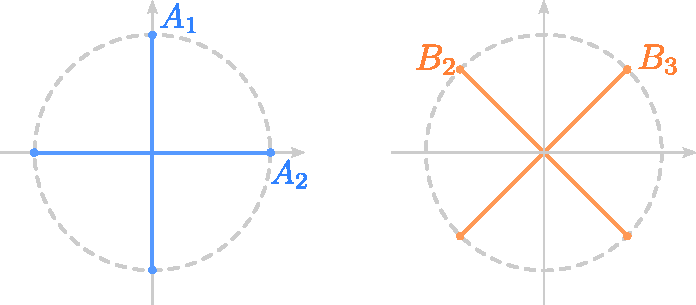
\includegraphics[width=0.7\textwidth]{lesson10/10-3_bases_CHSH.pdf}
    \caption[E91 - CHSH bases]{When the basis choices don't coincide the measurement outcomes can be still used for the CHSH test.}
    \label{fig:10-3_e91_example_CHSH}
\end{figure}

% So, visually it does correspond to Alice looking for cases where she measures in the $Z$ basis and in the $X$ basis, and Bob measures in this rotated bases B2 and B3, and then they use those measurement results to compute the following expression, which is just the sum of expectation values where Alice measured B1 and Bob measured B2, Alice measured A1 and Bob measured B3, and so on. 
This way, they don't need to discard information as was done in BB84. They get to use the information to calculate either the secret correlated key or the CHSH violation. (See the exercises for more on this.) If they obtain a CHSH correlation function such that $\mathcal{S} \leq 2$, they say "okay, we cannot conclude whether or not we have an entangled state, but it's safer to just abort."  If they have a $\mathcal{S} > 2$, then they conclude, "yes, we are sharing an entangled state, therefore we can proceed with the protocol." Remember, we said that monogamy of entanglement ensures that if they have an entangled state, then Eve cannot be not strongly correlated with either of them.  In particular, if Alice and Bob have a maximally entangled state, then Eve is not correlated with them at all, so they are looking for as strong a violation as they can get.

So far, we have considered the case where everything was ideal, with no noise. But what happens in real life, where noise is always present? How does noise affect our QKD protocols? In real life, the CHSH value will not equal exactly $2\sqrt{2}$, as we saw in Tab.~\ref{tab:chsh-calculation}.  Moreover, Alice and Bob will not be able to generate a perfectly correlated key, meaning that either noise or the tinkering of Eve will introduce some inconsistencies into the key. Even if Eve is not trying to actively eavesdrop and disrupt the protocol, still, due to inherent noise in the system, these keys will not be perfectly correlated.

Alice and Bob have to decide on the acceptable security risk even if the keys are not perfectly correlated. They have to agree, "Okay, if the correlation is not a hundred percent, but it's very close to hundred percent, we can still use this to do something useful, and use it for a secret communication." If they agree to this in principle, then they have to engage in two more protocols. One is called  \emph{information reconciliation}, which takes the initial secret key that's not perfectly correlated and produces a more correlated key.  It increases the correlation between the secret keys obtained hy Alice and Bob.  As cryptosystems generally are designed so that a single bit's difference in the keys changes half of the bits in the encrypted message, they require that exactly the same key be used at both ends.  Alice and Bob also can perform something known as \emph{privacy amplification}, where they take their generated secret key and produce a shorter key which is more secure. They are basically trying to eliminate any possible correlation with Eve.

So, which protocol is better, BB84 or E91? One is based on the indistinguishability of single photons prepared in non-orthogonal bases, and the other uses entanglement. In particular, we care about the security of both of these protocols. Let's compare from the point of view of when the secret key is generated.

In the case of the BB84 protocol, candidate bits for the key are generated when Alice generates her random string right at the beginning of the protocol. Remember, she generates two random $n$-bit strings. One string encodes the information about the basis of preparation, and the other encodes the bits themselves. So if Alice chooses the $Z$ basis, the state she prepares is a \ket{0} or a \ket{1}, whereas if she chooses the $X$ basis, she prepares a \ket{+} or a \ket{-}. So the secret key (or an extended form of it before photons are lost and their corresponding bits are discarded) exists right from the beginning, before any communication between Bob and Alice takes place.

That means that a clever Eve can actually find a way to obtain some information about this secret bit string. In particular, you can consider a very paranoid scenario where the random number generator that Alice is using to generate a random bit string was actually produced by Eve and is in some way correlated with Eve, therefore whatever random bit string that the device produces, that information gets passed on to Eve. We saw at the beginning of this chapter that that poses a huge security risk for BB84 protocol.

In contrast, in the E91 protocol, the secret key is really generated after the entangled pairs of qubits are measured, not when Eve produces those entangled pairs, not when they arrive at Alice and Bob, but only after Alice and Bob measure them in their random bases. In that sense, we can say that the key is unconditionally secure, and we see that entanglement is very essential for security.

Let's conclude this chapter by talking about some entanglement-based QKD experiments. We saw in BB84 that there were network testbeds for single photon QKD networks, however the development of entanglement-based QKD is not as advanced but it exists at the level of establishing a secret key over a single link. One such experiment was performed over free space, meaning that the entangled photons traveled through through air.  This experiment was done over a distance of 144 kilometers between La Palma and Tenerife, two islands in the Canary Islands. Photon pairs were produced by the spontaneous parametric down-conversion (SPDC)\index{spontaneous parametric down-conversion (SPDC)} process which we saw in Sec.~\ref{sec:4-4_spdc}. The qubit was encoded in the polarization of the photons. The obtained CHSH value, $\mathcal{S} =2.508$, was quite a substantial amount above the classical value of 2, giving a strong CHSH violation.

A different, more recent experiment was done over a distance of hundreds of kilometers, but it was done in a lab and over optical fiber. The fiber was very long and it was wound around a spool in the lab.  Two distances were tested. The  first distance was 311 kilometers over standard fiber, and the other distance was 404 kilometers over an ultra-low loss fiber.  In this experiment, the obtained bit rate for the secret key was of the order of $10^{-3}$ bits per second for the shorter distance, or $10^{-4}$ bits per second for the longer distance. These bit rates don't actually include the information reconciliation and privacy amplification parts of a full protocol, so if we wish to use this scheme in real life, we would actually have to add these functions, which would further lower the bit rate.

Another fantastic experiment was performed with satellites, where the satellite actually distributed entangled pairs between two ground stations, and the ground stations were 1,120 kilometers apart. Remember, we said that the light travels in a straight line, whereas using a satellite we can overcome the complication of curved earth's surface to establish a quantum key over much longer distances. So the total distance was over one thousand kilometers, and the measured CHSH value was $\mathcal{S} = 2.56$, again showing a strong CHSH violation. The obtained bit rate was 0.12 bits per second. Now, one could ask the question, what if we actually used a single fiber to connect these two ground stations? Well, the paper that reported these results estimated that the fiber would have been around eleven orders of magnitude less efficient than using the satellites, which is quite incredible.  At the beginning of this chapter, we discussed the security-related reason for preferring E91 to BB84; arguably, an even bigger reason is simply the loss in fiber, which we will address in Ch.~\ref{sec:11_long-distance} and beyond.

This concludes our discussion of quantum key distribution protocols as a key use of quantum effects in communication systems.

\newpage
\begin{exercises}
\exer{
In E91, Alice and Bob each have three choices of measurement basis, which they are expected to select randomly.  We described how six different pairs of choices are used to generate the secret key and to calculate the CHSH inequality to check for the presence of an eavesdropper.
% A2B1, A3B1, A3B2 aren't mentioned.  A2B1 is orthogonal bases and should be just random. A3B1 and A3B2 are equivalent to two of the other measurements, and could be included in a CHSH calculation, with appropriate normalization.
\subexer{
Sharp-eyed readers may have recognized that, in the explanation, we neglected three choices of basis.  Which ones did we not mention, and why?  What should be done with the data collected when those bases are chosen?
}
\subexer{Taking into account the answer to the prior question, what fraction of total measurements are dedicated to key generation, and what fraction to CHSH testing?}
}

\exer{We described E91 using \ket{\Psi^+} Bell pairs.  Does anything change if we use a different kind of Bell pair?}

\exer{Calculate the value of $\mathcal{S}$ for a CHSH inequality based on \rdv{add some data here, whether real or fake.  Maybe one real one each from an IBM machine and the QuTools?}.}

\exer{If the success probability for transmitting a photon through $1,120$km of fiber is $10^{-14}$, determine the loss per kilometer, in dB.}

\exer{On the Bloch sphere, the four basis choice angles for CHSH are 45\degree apart.  Derive an expression for the maximum $\mathcal{S}$ value as a function of that angle, assuming the four bases are all the same distance apart.  Prove that the canonical choice of 45\degree is optimal.}

\end{exercises}

\newpage
\section*{Quiz}
  \addcontentsline{toc}{section}{Quiz}

% \section{Learning more}

\section*{Further reading for chapters 8-10}
  \addcontentsline{toc}{section}{Further reading for chapters 8-10}

Anton Zeilinger, Alain Aspect and John Clauser were awarded the 2022 Nobel Prize in Physics for their experimental demonstrations of the existence of entanglement, with teleportation being referenced indirectly.

A good, popular science treatment of the history of this area is \emph{The Age of Entanglement}, by Louisa Gilder.

chapter 8

This chapter introduced one the most fundamental protocols of quantum communication. “Mike \& Ike” Chapter 1 goes through the mathematics of the protocol. The original paper is a great read and we highly recommend it:

Charles H. Bennett, Gilles Brassard, Claude Crépeau, Richard Jozsa, Asher Peres, William K. Wootters, Teleporting an unknown quantum state via a dual classical and Einstein-Podolski-Rosen Channels, Physical Review Letters 70, 1895 (1993).

chapter 9

An enlightening discussion of the BB84 protocol can be found in Chapter 12 of “Mike \& Ike” along with some exercises that will deepen your understanding of the protocol.
The original paper can be found here:

Charles H. Bennett, Gilles Brassard, Quantum cryptography: Public key distribution and coin tossing, Theoretical Computer Science 560, 7 (2014).

For a further discussion of classical cryptography aimed at those working in quantum computing, see the forthcoming paper "What Every Quantum Researcher and Engineer Should Know about Classical Cryptography", by Van Meter and Aono.  Portions of this paper are available on Van Meter's blog.

chapter 10

Entanglement-based QKD was first introduced in:

Artur K. Ekert, Quantum cryptography based on Bell’s theorem, Physical Review Letters 67, 661 (1991).

This paper is unfortunately behind a paywall but you should be able to access it through your university’s library system.
Brief discussion of entanglement-based QKD can be also found in Chapter 12 of “Mike \& Ike”.

The exact security statistics necessary for effective QKD protocols, whether BB84 or E91, are a complex matter.  Information reconciliation and privacy amplification are major research topics in their own right. A paper on the topic for ambitious learners is \rdv{YYY}.